%!TEX root = Constructive Alignment for Introductory Programming.tex

\chapter{Constructively Aligned Introductory Programming Curriculum} % (fold)
\label{cha:example_impl}

\graphicspath{{Figures/CAIntroProg/}}

\cref{cha:approach} proposed an approach to delivering constructively aligned introductory programming unit based upon the principles from \cref{cha:guiding_principles}. The proposed apporach makes uses portfolio assessment, with an objects-later apporach that divides the programming content across two introductory programming units. This chapter provides an example implementation of this approach, demonstrating how the principles from \cref{cha:guiding_principles} and the approach from \cref{cha:approach} can be realised in a programming curriculum.

Sections of this chapter relate to the two introductory programming units: introductory programming, and object oriented programming. For each of these units the subsections are ordered to follow the processes from \cref{cha:approach}. First we outline the design of the intended learning outcomes, and the construction of the assessment criteria. This is followed by examples of the various teaching and learning activities and resources developed in implementing this curriculum.  


\section{Introductory Programming} % (fold)
\label{sec:introductory_programming}

\subsection{Aims for Introductory Programming} % (fold)
\label{ssub:intro:aims}

The aim of Introductory Programming is to introduce students to programming and software development fundamentals. While focusing on developing depth in this area, the wholistic nature of the portfolio assessment approach means that programming is placed in the context of software development in general. As a result, this unit will touch on a number of areas.


% subsubsection aims (end)

\subsection{Defining Intended Learning Outcomes} % (fold)
\label{sec:intro:intended_learning_outcomes}

\subsubsection{Influencing Factors} % (fold)
\label{ssub:influencing_factors}

\begin{figure}[htbp]
	\centering
	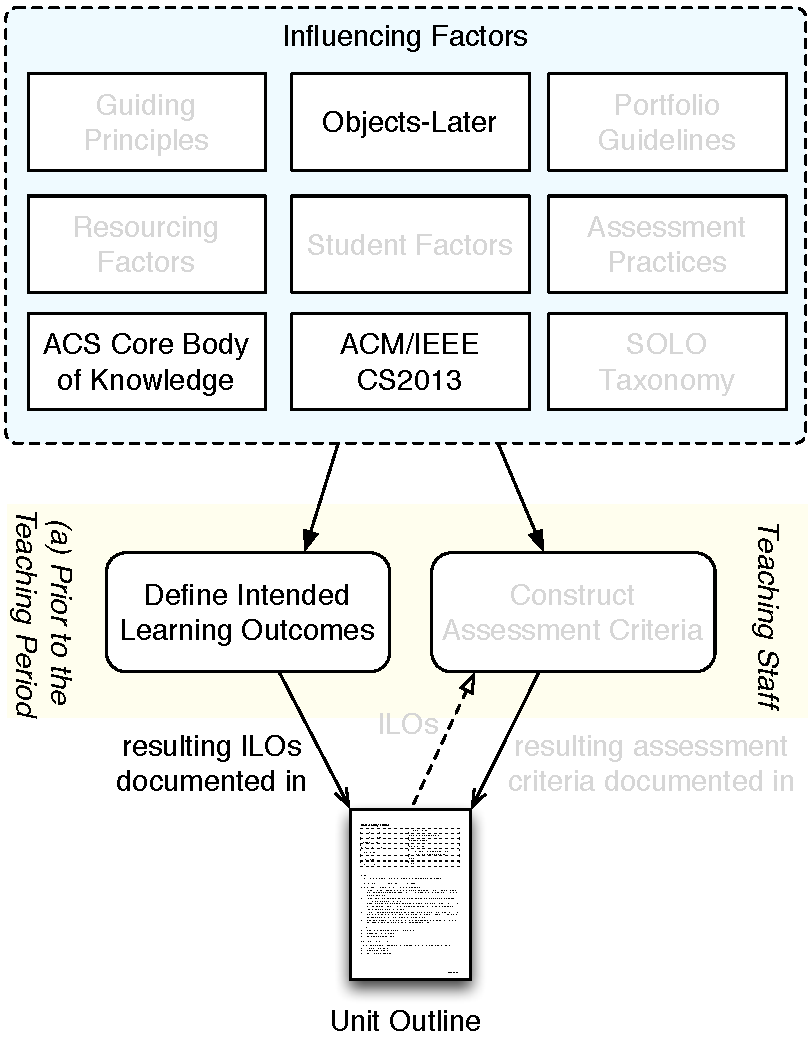
\includegraphics[width=0.7\textwidth]{ILOFactors}
	\caption{Factors that influence the defining of a unit's intended learning outcomes, and the construction of assessment criteria. \fref{fig:defining_ilos}}
	\label{fig:defining_ilos_intro}
\end{figure}

The Association for Computing Machinery and IEEE Computer Society 2013 Computer Science Curriculum \cite{CSC2013} outlines a number of areas to be covered in a Computer Science curriculum. In terms of this model curriculum, the Introductory Programming Unit presented here touched upon a range of areas, as shown in the following list. The primary focus was on the Software Development Fundamentals, but also integrated a number of other areas.

\begin{itemize}[noitemsep,nolistsep]
	\item AL/Algorithmic Strategies: students were introduced to divide-and-conquer, and the idea of recursive backtracking.
	\item AL/Fundamental Data Structures and Algorithms: all students programmed simple numeric algorithms, sequential search, and basic sorting.
	\item CN/Processing: fundamental programming concepts were covered in depth, including algorithms,  implementing algorithms in code, and processes in the software development lifecycle.
	\item DS/Basic Logic: students used truth tables to learn to evaluate boolean expressions.
	\item GV/Fundamental Concepts: applications of computer graphics, double buffering and animation were covered to make programming more interactive.
	\item GV/Geometric Modelling: Optional tasks allowed students to explore procedurally generated models (fractals).
	\item HCI/Programming Interactive Systems: students developed code to manage events and user interactions.
	\item PL/Basic Type Systems: students explored the use of a range of basic types, along with the definition of custom enumerated and record types.
	\item PL/Language Translation and Execution: students are introduced to the topics of compilers and interpreters, as well as run-time layout of memory (call-stack, heap, static data), and manual memory management.
	\item SDF/Algorithms and Design: students were introduced to the concept of algorithms, problem solving using divide-and-conquer, abstraction and program decomposition.
	\item SDF/Fundamental Programming Concepts: students used programming language syntax, develop programs that contained statements, expressions, use variables, simple input and output operations, with conditional control flow, included functions, various parameter passing techniques, and were introduced to the concept of recursion.
	\item SDF/Fundamental Data Structures: programs students implemented made use of arrays, record structures, strings and basic string processing, and students implemented a simple linked list.
	\item SDF/Development Methods: program comprehension was central to the unit, with basic details of program correctness being introduced. Students were also required to use basic refactoring techniques to restructure code, and program tracing was covered as a debugging technique.
	\item SE/Software Processes: students used an iterative software development process model, and were introduced to the phases of the software development lifecycle. 
	\item SE/Software Design: students were introduced to the principles of the structured design paradigm, and used these principles in the design and development of the programs they created.
	\item SE/Software Construction: coding standards, and defensive coding practices were introduced to students.
	\item SP/Professional Ethics: students develop skills in professional practice including self assessment, reflective practice, computer fluency, and general approach to life-long learning.
	\item SP/Professional Communication: to demonstrate their understanding students were required to read, understand and communicate technical material using clear language and visual mediums.
\end{itemize}

The Australian Computer Society (ACS) documented the ICT profession and associated body of knowledge \cite{Gregor:2008}, which indicated graduates should develop both skills and knowledge as part of their undergraduate education. The knowledge area is divided into three aspects: a core body of knowledge, role specific knowledge and complementary knowledge. The introductory programming unit develops student's skills and knowledge.

The skills component of the ACS document drew upon the skills documented in the Skills Framework for the Information Age (SFIA). In terms of the SFIA \cite{SFIA:2011} the Introductory Programming unit aimed to contribute to the development of programming and software development skills to a Level 2, \emph{assist}, standard. This indicates that students need to demonstrate the ability to design, code, test, correct, and document simple programs, and indicates that students are able to assist with the development of larger software solutions.

The ACS divides the core body of knowledge into six areas: problem solving, professional knowledge, technology building, technology resources, service management and outcomes management.

% subsubsection influencing_factors (end)

\subsubsection{Intended Learning Outcomes} % (fold)
\label{ssub:intended_learning_outcomes}

% subsubsection intended_learning_outcomes (end)

Introductory Programming used a procedures-first approach, and focused on the structured programming principles of organising code using \emph{sequence}, \emph{selection} and \emph{repetition}. Students learnt to use functional and modular decomposition to break problems down, and implement solutions using functions and procedures. Data was managed using arrays and custom data types. Pointers and memory management were introduced. Various forms of parameter passing were covered, including pass-by-value and pass-by-reference. Weaved through this was an iterative development process, a focus on writing clear and legible code, and other good programming practices. In addition to writing code, students learnt to read code for the debugging purposes, and to demonstrate their ability to interpret other peoples code. All of this is captured in the intended learning outcomes for Introductory Programming:
\begin{enumerate}[noitemsep,nolistsep]
	\item Apply code reading and debugging techniques to analyse, interpret, and describe the purpose of program code, and locate within this code errors in syntax, logic, and/or good practice.
	\item Describe the principles of structured programming, relate these to the syntactical elements of the programming language used, and the way programs are developed using this language.
	\item Construct small programs, using the programming languages covered that include the use of arrays, functions and procedures, parameter passing with call by value and call by reference, custom data types, and pointers.
	\item Use modular and functional decomposition to break problems down functionally, represent the resulting structures diagrammatically, and implement the structure in code as functions and procedures.
\end{enumerate}

% section introductory_programming (end)






\subsection{Object Oriented Programming} % (fold)
\label{sub:object_oriented_programming}

% subsection object_oriented_programming (end)

Object Oriented Programming takes students who have completed Introductory Programming and introduces them to the object oriented programming paradigm. Students will learn about the core principles of object oriented programming, and how these can be used to create object oriented programs. They will develop programs using integrated development environments, including  unit testing tools. Students will be introduced to visual ways of communicating object oriented designs using the Unified Modelling Language \cite{Fowler:2004}, including both class diagrams and sequence diagrams. Design patterns and heuristics will be used to provide students with a means of evaluating the quality of their designs. As with Introductory Programming students will use a iterative development process. The intended learning outcomes for Object Oriented Programming are:
\begin{enumerate}
	\item Explain the principles of the object oriented programming paradigm specifically including abstraction, encapsulation, inheritance and polymorphism, and explain how these principles are used to create object oriented programs.
	\item Design, develop, test, and debug object oriented programs, using an integrated development environment.
	\item Select and use appropriate collection classes, from the language's class library, to manage collections of multiple objects.
	\item Construct appropriate diagrams and textual descriptions to communicate the static structure and dynamic behaviour of an object oriented solution.
	\item Apply accepted good practices related to the construction of object oriented programs.
\end{enumerate}
% subsection intended_learning_outcomes (end)


Pascal \cite{Becker:2002}



% section concepts_in_introductory_programming (end)

\section{A Simplified Taxonomy to Frame Programming Concepts} % (fold)
\label{sec:a_simplified_taxonomy_to_frame_programming_concepts}

% section a_simplified_taxonomy_to_frame_programming_concepts (end)

\section{Introductory Programming, Procedures First} % (fold)
\label{sec:introductory_programming_procedures_first}

% section introductory_programming_procedures_first (end)

\section{Using Multiple Languages to Focus on Concepts} % (fold)
\label{sec:using_multiple_languages_to_focus_on_concepts}

% section using_multiple_languages_to_focus_on_concepts (end)

% chapter constructively_aligned_introductory_programming_curriculum (end)